\documentclass{beamer}
\usepackage[utf8]{inputenc}
\usepackage{graphicx}
\usepackage{amsmath}
\usepackage{listings}
\usepackage{xcolor}
\usepackage{hyperref}
\hypersetup{
    colorlinks=true,
    linkcolor=blue,
    filecolor=magenta,
    urlcolor=cyan,
}

\title{Finding Zeroes for Polynomials using}
\subtitle{Newton-Raphson and Bisection Method}
\author{Scientific Programming Project}

\begin{document}

\frame{\titlepage}

\begin{frame}{Project Overview}
\begin{itemize}
    \item Goal: Find all real roots of a polynomial \( p(x) \in \mathbb{R}[x] \)
    \item Implement Newton-Raphson and Bisection methods
    \item Python and Haskell implementations
    \item Compare implementations with built-in Numpy and HMatrix implementations
    \item Runtime must be under 8 seconds
\end{itemize}
\end{frame}

\begin{frame}{Algorithm: Newton-Raphson}
\begin{itemize}
    \item Iterative method using first derivative and an initial guess
    \item Update rule: \( x_{n+1} = x_n - \frac{f(x_n)}{f'(x_n)} \)
    \item Fast convergence if initial guess is close
    \item Time Complexity is O(log(log(n)))
    \item But... Can fail if derivative is zero or initial guess is poor\newline Can exceed out of bounds [a, b]
\end{itemize}
\end{frame}

\begin{frame}{Algorithm: Bisection Method}
\begin{itemize}
    \item Bracketed root-finding method
    \item Halves interval \([a, b]\) until $width < \epsilon\ $ \
    \item Always converges if root is in interval
    \item Time Complexity is O(log(n)). Slower than Newton-Raphson.
\end{itemize}
\end{frame}

\begin{frame}{Hybrid Approach}
\begin{itemize}
    \item The hybrid approach is supposed to find a single root in an interval [a, b], wherein f sustains $f(a)*f(b) < 0 $
    \item Assumptions - Each root x of polynomial f(x) ensures either f'(x) = 0 or x is between two roots of f'(x)
    \item Use Newton-Raphson to find roots in respect to the defined tolerance $\epsilon\ $ \
    \item If bounds are exceeded, fallback to Bisection
    \item \textbf{Finds a single root in a given interval [a, b]}
\end{itemize}
\end{frame}


\begin{frame}{Optimization Techniques*****}
\begin{itemize}
    \item \textbf{Normalization:} Scaled polynomial by max coefficient to avoid overflow
    \item \textbf{***Overflow Handling:} Evaluated $p(1/x)$ instead of $p(x)$ for $|x| > 1$
    \item \textbf{Used solutions from lectures:} Used the best solutions of polyVal, polyDiv and derivative from the lectures.
    \item \textbf{Redundant Pythonic loops:} Avoided unnecessary usage of Pythonic loops, resorted to NumPy vectorization techniques.
    \item \textbf{***Derivative Reuse:} Computed derivative once and reused across Newton–Raphson and fallback methods
    \item \textbf{Early Exit:} Bisection returns immediately if endpoint is root
    \item \textbf{Bound Estimation:} Used Fujiwara's bound to limit root search space; using geometrical properties of polynomial roots
\end{itemize}
\end{frame}


\begin{frame}{Polynomial Root Bounds}
\begin{itemize}
    \item Used bounds to limit root search interval
    \item Compared Cauchy, Kojima, and Fujiwara bounds
    \item \textbf{Fujiwara bound was fastest in integration with the hybrid approach}
\end{itemize}
\end{frame}

\begin{frame}{Fujiwara Bound}
\begin{itemize}
  \item Let $p(z)=a_n z^n + a_{n-1} z^{n-1} + \dots + a_0$ with $a_n\neq 0$.
  \item \textbf{Fujiwara’s bound:} every root $\gamma$ of $p$ satisfies
        \[
          |\gamma|\;\le\;
          2\max\Bigl\{
          \bigl|\tfrac{a_{n-1}}{a_n}\bigr|,
          \bigl|\tfrac{a_{n-2}}{a_n}\bigr|^{\frac12},
          \dots,
          \bigl|\tfrac{a_{1}}{a_n}\bigr|^{\frac1{n-1}},
          \bigl|\tfrac{a_{0}}{2a_n}\bigr|^{\frac1n}
          \Bigr\}.
        \]

  \item Fujiwara tightens Cauchy’s classical bound by reducing the factor on the constant term, giving us a generally sharper disk that contains all roots.
  \item If none of the coefficients vanish, Fujiwara is always sharper: each term in Fujiwara’s max is the \emph{geometric mean} of a prefix of Kojima’s terms, so the maximum can only decrease.
\end{itemize}
\end{frame}

\begin{frame}[fragile]{Python Runtime}
\texttt{Tolerance used: 1e-6, Polynomial: Provided CSV - 996 Coefficients and a free coefficient}
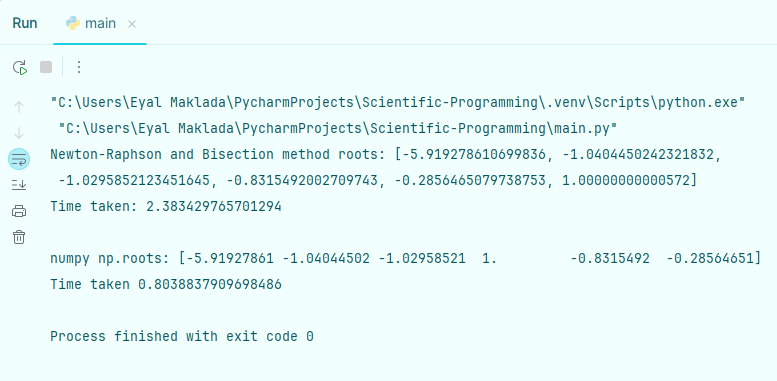
\includegraphics[width=1.0\textwidth]{python_runtime.png}
\end{frame}

\begin{frame}[fragile]{Haskell Runtime}
\texttt{Tolerance used: 1e-6, Polynomial: Provided CSV - 996 Coefficients and a free coefficient}
\includegraphics[width=1.0\textwidth]{haskell_runtime.png}
\end{frame}

\begin{frame}{Runtime Comparison}
\begin{itemize}
    \item Compared custom vs. built-in implementations
    \item Built-in methods: NumPy root finder for Python
    \item Custom methods: NumPy vectorization for Python, HMatrix for Haskell
    \item Our implementations stayed under 8s for all tests
    \item Differences due to derivative accuracy, convergence criteria
\end{itemize}
\end{frame}

\begin{frame}{Runtime Comparison – Closer Look at Built-in Methods******}
\begin{itemize}
    \item Built-in implementations adaptively select methods:
    \begin{itemize}
        \item Uses Newton–Raphson if $f'(x)$ is provided - quadratic convergence rate
        \item Else it Falls back to Secant method - sub-quadratic convergence rate
        \item Uses Halley’s method if $f''(x)$ is provided - cubic convergence rate
        \item See Docs: \href{https://docs.scipy.org/doc/scipy-0.14.0/reference/generated/scipy.optimize.newton.html}{SciPy.optimize.newton}
    \end{itemize}


    \item \textbf{Why NumPy (\texttt{np.roots}) is faster:}
    \begin{itemize}
        \item Uses eigenvalue decomposition of the companion matrix
        \item Backed by low-level Fortran libraries (e.g., LAPACK)
        \item Executes fully in compiled code (no Python loop overhead)
        \item Optimized for dense, fixed-size numeric arrays
    \end{itemize}

\end{itemize}
\end{frame}

\begin{frame}{Conclusion}
\begin{itemize}
    \item Hybrid root-finding is accurate and relatively fast
    \item Fujiwara bound provided best performance
    \item Python and Haskell both effective with vectorization; Obviously Haskell more so
    \item Differences from built-in implementations are explainable and expected
\end{itemize}
\end{frame}

\end{document}